%%
%% Copyright 2007-2020 Elsevier Ltd
%%
%% This file is part of the 'Elsarticle Bundle'.
%% ---------------------------------------------
%%
%% It may be distributed under the conditions of the LaTeX Project Public
%% License, either version 1.2 of this license or (at your option) any
%% later version.  The latest version of this license is in
%%    http://www.latex-project.org/lppl.txt
%% and version 1.2 or later is part of all distributions of LaTeX
%% version 1999/12/01 or later.
%%
%% The list of all files belonging to the 'Elsarticle Bundle' is
%% given in the file `manifest.txt'.
%%
%% Template article for Elsevier's document class `elsarticle'
%% with harvard style bibliographic references

% For submission:
\documentclass[final,5p,times,twocolumn,authoryear]{elsarticle}

%% Use the option review to obtain double line spacing
% \documentclass[authoryear,preprint,review,12pt]{elsarticle}

%% Use the options 1p,twocolumn; 3p; 3p,twocolumn; 5p; or 5p,twocolumn
%% for a journal layout:
%% \documentclass[final,1p,times,authoryear]{elsarticle}
%% \documentclass[final,1p,times,twocolumn,authoryear]{elsarticle}
%% \documentclass[final,3p,times,authoryear]{elsarticle}
%% \documentclass[final,3p,times,twocolumn,authoryear]{elsarticle}
%% \documentclass[final,5p,times,authoryear]{elsarticle}
%% \documentclass[final,5p,times,twocolumn,authoryear]{elsarticle}

%% For including figures, graphicx.sty has been loaded in
%% elsarticle.cls. If you prefer to use the old commands
%% please give \usepackage{epsfig}

%% The amssymb package provides various useful mathematical symbols
\usepackage{amssymb}
%% The amsthm package provides extended theorem environments
%% \usepackage{amsthm}

%% The lineno packages adds line numbers. Start line numbering with
%% \begin{linenumbers}, end it with \end{linenumbers}. Or switch it on
%% for the whole article with \linenumbers.
%% \usepackage{lineno}

\graphicspath{{figures/}}
% imports
\usepackage{xcolor}
\usepackage{hyperref}
\hypersetup{
    colorlinks=true,
    linkcolor=black,
    filecolor=black,
    urlcolor=navy,
    citecolor=black,
}
\urlstyle{same}

% Packages / projects / programming
\newcommand{\package}[1]{\texttt{#1}}
\newcommand{\acronym}[1]{{#1}}
\newcommand{\github}{\textsl{GitHub}}
\newcommand{\python}{\textsl{Python}}
\newcommand{\jax}{\package{JAX}}
\newcommand{\agama}{\package{Agama}}
\newcommand{\gala}{\package{gala}}

% Missions
\newcommand{\gaia}{\textsl{Gaia}}
\newcommand{\hipparcos}{\textsl{HIPPARCOS}}
\newcommand{\dr}[1]{\acronym{DR}#1}
\newcommand{\apogee}{\acronym{APOGEE}}
\newcommand{\sdss}{\acronym{SDSS}}
\newcommand{\sdssiv}{\acronym{SDSS-IV}}

% Stats / probability
\newcommand{\given}{\,|\,}
\newcommand{\norm}{\mathcal{N}}
\newcommand{\pdf}{\textsl{pdf}}

% Maths
\newcommand{\dd}{\mathrm{d}}
\newcommand{\deriv}[2]{\frac{\mathrm{d}{#1}}{\mathrm{d}{#2}}}
\newcommand{\dderiv}[2]{\frac{\mathrm{d^2}{#1}}{\mathrm{d}{#2}^2}}
\newcommand{\Deriv}[2]{\frac{\mathrm{D}{#1}}{\mathrm{D}{#2}}}
\newcommand{\pderiv}[2]{\frac{\partial {#1}}{\partial {#2}}}
\newcommand{\ppderiv}[2]{\frac{\partial^2 {#1}}{\partial {#2}^2}}
\newcommand{\transpose}[1]{{#1}^{\mathsf{T}}}
\newcommand{\inverse}[1]{{#1}^{-1}}
\newcommand{\argmin}{\operatornamewithlimits{argmin}}
\newcommand{\mean}[1]{\left< #1 \right>}

% Non-scalar variables
\renewcommand{\vec}[1]{\ensuremath{\bs{#1}}}
\newcommand{\mat}[1]{\ensuremath{\mathbf{#1}}}

% Units:
% Workaround for siunitx + AASTeX
% https://tex.stackexchange.com/questions/192610/use-emulateapj-aastex-with-siunitx
\usepackage{savesym}
\savesymbol{tablenum}
\usepackage{siunitx}
\ifdefined\unit\else
  \ifdefined\NewCommandCopy
    \NewCommandCopy\unit\si
  \else
    \NewDocumentCommand\unit{O{}m}{\si[#1]{#2}}
  \fi
\fi
\restoresymbol{SIX}{tablenum}
\DeclareSIUnit\year{yr}
\DeclareSIUnit\parsec{pc}
\DeclareSIUnit\mag{mag}
\DeclareSIUnit\Msun{M_\odot}
\DeclareSIUnit\msun{M_\odot}
\DeclareSIUnit\Rsun{R_\odot}
\DeclareSIUnit\mas{mas}
\newcommand{\mas}{\unit{\milli\arcsecond}}
\newcommand{\muas}{\unit{\micro\arcsecond}}
\newcommand{\kms}{\unit{\km\per\s}}
\newcommand{\masyr}{\unit{\mas\per\year}}
\newcommand{\kpc}{\unit{\kilo\parsec}}
\newcommand{\usurfdens}{\unit{\msun.\parsec^{-2}}}
\newcommand{\uvoldens}{\unit{\msun.\parsec^{-3}}}

% Misc. formatting
\newcommand{\bs}[1]{\boldsymbol{#1}}

% Astronomy
\newcommand{\abun}[2]{\ensuremath{{[\mathrm{#1}/\mathrm{#2}]}}}
\newcommand{\feh}{\abun{Fe}{H}}
\newcommand{\afe}{\abun{\alpha}{Fe}}
\newcommand{\mgfe}{\abun{Mg}{Fe}}
\newcommand{\logg}{\ensuremath{\log g}}
\newcommand{\Teff}{\ensuremath{T_{\textrm{eff}}}}
\newcommand{\vsini}{\ensuremath{v\,\sin i}}

% Dynamics
\newcommand{\df}{\acronym{DF}}
\newcommand{\zmax}{\ensuremath{z_{\textrm{max}}}}

% TO DO
\newcommand{\todo}[1]{{\color{red} TODO: #1}}
\newcommand{\placeholder}[1]{{\color{purple} #1}}


\journal{New Astronomy Reviews}

\begin{document}

\begin{frontmatter}

%% Title, authors and addresses

%% use the tnoteref command within \title for footnotes;
%% use the tnotetext command for theassociated footnote;
%% use the fnref command within \author or \affiliation for footnotes;
%% use the fntext command for theassociated footnote;
%% use the corref command within \author for corresponding author footnotes;
%% use the cortext command for theassociated footnote;
%% use the ead command for the email address,
%% and the form \ead[url] for the home page:
%% \title{Title\tnoteref{label1}}
%% \tnotetext[label1]{}
%% \author{Name\corref{cor1}\fnref{label2}}
%% \ead{email address}
%% \ead[url]{home page}
%% \fntext[label2]{}
%% \cortext[cor1]{}
%% \affiliation{organization={},
%%            addressline={},
%%            city={},
%%            postcode={},
%%            state={},
%%            country={}}
%% \fntext[label3]{}

\title{Stellar Streams in the Gaia Era}

%% use optional labels to link authors explicitly to addresses:
%% \author[label1,label2]{}
%% \affiliation[label1]{organization={},
%%             addressline={},
%%             city={},
%%             postcode={},
%%             state={},
%%             country={}}
%%
%% \affiliation[label2]{organization={},
%%             addressline={},
%%             city={},
%%             postcode={},
%%             state={},
%%             country={}}

\author[ociw]{Ana~Bonaca}
\author[cca]{Adrian~M.~Price-Whelan}

\affiliation[ociw]{organization={The Observatories of the Carnegie Institution for Science},
            addressline={813 Santa Barbara Street},
            city={Pasadena},
            postcode={91101},
            state={CA},
            country={USA}}

\affiliation[cca]{
    organization={Center for Computational Astrophysics, Flatiron Institute},
    addressline={162 Fifth Ave.},
    city={New York},
    postcode={10010},
    state={NY},
    country={USA}
}


\begin{abstract}
- streams, tidal debris, useful for tracing hierarchical assembly, dark matter
- in the Milky Way, the Gaia mission, providing astrometry and spectrophotometry for billions of stars, fundamentally changed the landscape
- we discuss three main revolutions:
-- number of streams increased by an order of magnitude, now have a population of 100 (New streams and methods for discovery thanks to new kinds of data)
-- orbital histories (including hierarchical associations between streams)
-- Stream features are abundant (revealed at low surface brightness)
Implications heralding exciting times ahead!
-- pragmatic: Due to more secure membership probabilities, follow-up now more efficient so the chemistries now becoming more readily available
-- Due to large number of streams, transitioning from stamp-collecting to population studies
-- All of this will need improved theoretical modeling of the new Gaia discoveries
\end{abstract}

% %%Graphical abstract
% \begin{graphicalabstract}
% %\includegraphics{grabs}
% \end{graphicalabstract}
%
% %%Research highlights
% \begin{highlights}
% \item Research highlight 1
% \item Research highlight 2
% \end{highlights}

\begin{keyword}
%% keywords here, in the form: keyword \sep keyword

%% PACS codes here, in the form: \PACS code \sep code

%% MSC codes here, in the form: \MSC code \sep code
%% or \MSC[2008] code \sep code (2000 is the default)

\end{keyword}

\end{frontmatter}

%% \linenumbers

%% main text
\section{Introduction}
\label{sec:intro}
% AB
% storytelling prose

- what happens when two galaxies approach (toomre)
- what happens to a dwarf galaxy when it approaches a more massive galaxy
- theory of tidal stripping
-- Shell vs stream, radial vs tangential
-- Dwarf vs. globular cluster

- much of this theory developed bc stuff seen in arp's catalog?
- where observed: extragalactic -- interacting galaxies, streams, shells
- took some time to discover in the mw, looking from the inside
- mw halo discoveries in new surveys: hipparcos (phase-mixed), 2MASS, SDSS (coherent)

- Mergers common, expected in dm universe
- tracers in the MW halo, evidence of hierarchical galaxy formation, predicted in the dm paradigm
- but also more direct tracer of dm: distribution on large, galactic \citep{varghese, bonaca:2014}, and small, subgalactic, scales \citep{johnston, ibata}

- the longest stream to date sgr, traced to wrap around more than 360deg \citep{majewski, belokurov}
- almost great circle -- potential close to spherical
- with first rvs: prolate \citep{helmi}
- more detailed look at sky positions: great circle precession -> oblate \citep{johnston}
- more flexible model employed to fit both: triaxial \citep{law, lmj, deg}
- kinematics key \citep{bh:2018, nibauer, pearson}
- But kinematics hard observationally, need spectroscopy, more time-consuming, in addition targets are sparse \citep{kuzma, etc}, so follow-up inefficient, even hard even beyond just the lack of appropriate observational capabilities
- proper motions in the halo possible with HST for bound satellite dwarf galaxies and globular clusters \citep{kallivayalil, vdmarel, sohn, watkins}
- but for streams only where fortuitously first epoch imaging available \citep{sohn}
- among the vast expanse of the MW sky, kinematic follow up of streams is highly inefficient

Even more alarmingly, although in retrospect perhaps not that surprisingly, similar analyses of other streams indicated that streams individually give a biased view of the halo.
The first such inkling came when \citet{pearson:2015} simulated tidal tails of the Palomar~5 globular cluster in the triaxial halo potential preferred by the Sagittarius stream, and found that the resulting Pal~5 model is significantly more dispersed than the observed stream \citep{odenkirchen:2001, rockosi:2002}.
Combined with the finding that a stellar disk in this potential model is unstable \citep{debattista:2013}, a triaxial halo was disfavored, at least in the inner Galaxy.
- naturally, a solution would be a simultaneous fit
- ideally with thin stellar streams, most constraining \citep{lux}
- GD-1 X Pal5, joint solution exists, but each stream pushing away \citep{bovy}
- indicates an ellipsoidal halo is too simplistic and we need a more complex model that captures \citep{halo_shapes, lowing}
- stream info indications that streams are local tracers, and that a more complex potential model could be constrained with more streams \citep{bh:2018}
- ideally, these streams would be at a range of distances, but large area photometric surveys tapped out at current depth
- and while deeper surveys always discovered more streams \citep{pandas, des}, their coverage is limited
In a modest number of stellar streams, we hit another limit to tracing dark matter in the Milky Way halo.

At the same time, progress was being made in constraining dark matter substructure.
Numerical experiments of cold dark-matter subhalos impacting stellar streams, both in idealized and cosmological settings, demonstrated that subhalos produce a range of observable features in streams, including variations in density, enhanced dispersion, stream folds, and stream track wiggles and asymmetries \citep{carlberg:2009, yoon:2011, ngan:2015, ngan:2016, sandford:2017}.
Across these studies, a stream underdensity, or a gap, was the most ubiquitous signature of a subhalo impact, so follow-up studies estimated the expected rates of subhalo-induced stream gaps \citep{carlberg:2012b, ngan:2014, erkal:2016, banik:2018}, as well as developed theoretical frameworks for inferring parameters of the impact from properties of individual gaps \citep{carlberg:2013b, erkal:2015a, erkal:2015b, helmi:2016, sanders:2016, koppelman:2021}.
A handful of seemingly high-confidence gaps were identified using SDSS and PAndAS photometry for streams discovered in the Milky Way and M31, respectively \citep{carlberg:2011, carlberg:2012, carlberg:2013, carlberg:2016b, carlberg:2016}, in broad agreement with the expected LCDM rates.
These findings motivated deeper imaging of these streams, which confirmed several prominent, degrees-wide gaps, but also revealed a density profile that is overall more uniform than that inferred from the shallower imaging \citep{ibata:2016, erkal:2017, bovy:2017, deboer:2018, bonaca:2020}.
This underlines the importance of securely identifying stream members from the foreground Milky Way stars, whose density variations could be mistaken for signatures of dark-matter subhalo impacts \citep{thomas:2016}.
Unfortunately, such deep photometry for all known streams is prohibitively expensive even with today's facilities.

By mid-2010s, we had a dozen streams discovered in the Milky Way, statistical inference methods developed and tested, but were no closer to knowing either the mass and shape of our dark matter halo, or its structure on small scales.
A prominent astronomer at an IAU Symposium 311 voiced frustration at this lack of progress by exclaiming ``Where is the beef with streams?!''.
As we now know, that moment in time was the very eve of a revolution awaiting the streams community, which started with the launch of the \gaia\ spacecraft in December 2013.
Conceived even before any stream had been discovered in the Milky Way \citep{lindegren:1993, battrick:1994, lindegren:1996}, \gaia\ was designed to deliver \emph{``a census of the accurate positions, distances, space motions (proper motions and radial velocities), and photometry of all approximately one billion objects complete to $V=20$\,mag''} \citep{perryman:2001} --- precisely the measurements needed to break through the limits of stream studies.
The first three Data Releases from the \gaia\ mission unveiled the structure of our Galaxy in unprecedented detail \citep{babusiaux:2018, helmi:2018, katz:2018, antoja:2021, smart:2021, drimmel:2023, schultheis:2023}, including dwarf galaxies accreted and phase-mixed onto the Milky Way \citep{belokurov:2018, helmi:2018b, myeong:2019, naidu:2020}, as well as moving groups and dissolved star clusters in the Solar neighborhood \citep{antoja:2018, kawata:2018, ramos:2018, meingast:2019, roser:2019}.
All of these types of substructures can be considered streams, but since we couldn't do all of them justice in this review, we will focus on a subset of long, coherent stellar streams accreted in the Milky Way halo, which in the \gaia\ era became our most sensitive antennae for dark matter.

- for a sneak preview:
-- outline individual sections
-- identify key summary figures?
-- state we identify key opportunities for breakthroughs
-- reflect on the changes awaiting us in the future due to these discoveries in the concluding section


% % APW Note:
% - Make sure we note that the focus here is on streams accreted, not disk / star cluster
% streams. Or kinematic substructures in the local velocity field (e.g., moving groups, Hipparcos UV structure, etc.)

\section{Stream Discovery and Characterization in the \gaia\ Era}
\label{sec:discovery}
% APW
% Questions:
% - Table of streams? What should it have in it? Name, survey, discovery method,
%   validated / rediscovered with Gaia?
% - Photometric? Astrometry? Radial velocity? Distance tracers? Detailed abundances?
%   Stellar population / mass? Progenitor?

% Figure 1: Pedagogical figure showing matched filter on Gaia alone, GD-1 vs. astrometry
% - reproduction of figure from PW & Bonaca 2018
% Figure 2: All the streams in sky projection

\textbf{Summary}: Stellar streams inherently have low stellar densities and their
constituent stars are typically far from the Sun, making them difficult to observe and
study.
Finding and characterizing streams is therefore all about enhancing contrast over the
background Milky Way stars, either by filtering datasets to increase the relative
occurrence of stream stars in the filtered set, or by restricting the search to rare
tracers that are more likely to be found in streams than in the field (e.g., blue
horizontal branch stars that are common to old, metal-poor stellar populations).
The first streams and substructures around the Milky Way were discovered this way by
filtering photometric data for stars in the Galactic halo, where the background stellar
density is also inherently lower than in the disk or central galaxy.
Subsequent discoveries were made with deeper or wider-area photometry surveys, or by
combining photometric and spectroscopic information (e.g., radial velocities).
The largest explosion in the number of known streams has come only over the last few
years thanks to data from the \gaia\ Mission.
The astrometric data from \gaia\ has revolutionized our ability to find kinematic
sub-structures because it is now possible to combine photometric and kinematic data for
enormous samples of stars.
In this section, we summarize the methods used to find streams in the pre-\gaia\ era and
highlight new methods that are now possible thanks to the all-sky kinematic data
available from \gaia.
We provide a brief census and summary of the streams that have been published up to now,
but note that this is still an active area for discovery and characterization.
We also discuss the limitations of the \gaia\ data and the need for future astrometric
surveys to push our understanding of the Milky Way's stellar halo and its dark matter
content to fainter magnitudes and larger distances.

% TODO: need to work in distinction between "thin stream" -> globular cluster, and dwarf galaxy streams

\subsection{Before \gaia}

% TODO Cite: Many of Carl's papers, Mario Mateo Carbon stars in Sgr, Majewski Sgr, Belokurov, Ibata stuff
The first stellar streams discovered around the Milky Way --- the Sagittarius stream
(Sgr) and the Palomar 5 stream (Pal 5) --- were found in the late 1990s and early 2000s
as over-densities of stars that connect back to their progenitor systems (the
Sagittarius dwarf galaxy and the Palomar 5 globular cluster, respectively).
Sgr and Pal 5 have since become archetypes of two major observational and interpreted
types of streams: dwarf galaxy or ``wide'' streams as compared to globular cluster or
``thin'' streams.
These discoveries, and most of the halo stellar streams found through the early 2000's,
were found using photometry alone.
The advent of deep, wide-area, multi-band sky surveys (especially the Sloan Digital Sky
Survey, SDSS, and the Two Micron All Sky Survey, 2MASS) were crucial for this initial
phase of stream discovery.
The combination of wide-area coverage, well-calibrated photometry (CITE uber-calibration
and Hogg paper), and near-uniform depth across the survey footprints enabled
constructing detailed maps of the stellar density of the Milky Way halo.
Still, streams are relatively low-density features and are surpassed in number counts by
the foreground and background stellar populations in the Milky Way in sky density alone.
Stream search methods must therefore leverage careful selection of stars based on the
expected stellar populations in accreted systems using multi-band photometry.

The most effective method for using photometric data to identify streams is to apply a
``matched filter'' \citep{Rockosi:2002:MatchedFilterAnalysisTidal} to the color--magnitude distribution of stars
to preferentially select or up-weight stars that are likely to be distant and low
metallicity.\footnote{We remind the reader that the focus here is on stellar streams
from accreted dwarf galaxy or globular cluster progenitor systems, which are expected to
be old and metal poor.}
Matched filters can be used as a boolean selection (e.g., select all stars within some
region of color and magnitude defined by isochrones) or as a weighting function (e.g.,
weight all stars by the probability that they are near an isochrone for an old and
metal-poor stellar population).
To search for streams, the filtered data was typically then displayed in sky
coordinates, sometimes by making movies that step the filter in distance modulus, and
maps of stellar density were smoothed and visually inspected for curving or linear
over-densities of stars.
Automated detection methods were explored, but this was the early days for computer
vision and machine learning, and most stream discoveries (even through the 2010's) was
done by visual inspection.

% TODO: Yanny? Others for list of SDSS stream papers?
Even now, many (TODO: how many?) of the known streams were found using a matched filter
based on photometry, plus visual inspection.
For example, the GD-1 stream --- the first long, thin stream discovered without a clear
progenitor --- was initially found by \citet{Grillmair:2006-gd1} using a matched filter
on SDSS photometry with visual inspection of the resulting stellar density maps.
Matched filters were also critical for many early discoveries of streams with the SDSS
data \citep[e.g.,][]{Newberg:2002,Yanny:2003, Belokurov:2006, Grillmair:2006-orphan}.
This method has since been applied to many large photometric surveys, such as 2MASS,
Pan-STARRS (PS1; \citealt{todo}), the Dark Energy Survey (DES; \citealt{todo}), Search
for the Leading Arm of Magellanic Satellites (SLAMS; \citealt{todo}), the DECam Legacy
Survey  (DECaLS; \citealt{todo}), and many smaller-area surveys.
In all cases, this has led to new stream and halo substructure discoveries.
For example, from 2MASS \citep{Rocha-Pinto, GASS, Anticenterstream}, PS1
\citep{Bernard, Ophiuchus, others?}, DES \citep{Shipp:2018}, SLAMS \citep{Jethwa:2018},
and DECaLS \citep{Shipp:2021}. PANDAS
Table~\ref{todo} has a list of streams discovered ...

Many of the systematic searches for streams described above were done without
considering specific progenitor systems (i.e. globular clusters or dwarf galaxies).
The discovered streams were then subsequently either found to be without a clear
progenitor system, or were associated with known systems based on their location in the
sky and/or their kinematics \citep{todo}.
However, some searches were specifically designed to find streams associated with known
globular clusters or dwarf galaxies \citep{Grillmair:1990, todo} using photometry around
these systems.
With the exception of the striking tidal tails around the Pal 5 globular cluster
\citep{Odenkirchen:2002} and the faint stream associated with NGC 5466
\citep{Grillmair:2006-ngc5466}, most of these searches were unsuccessful or only found
evidence for very low-density tidal tails based on the presence of small numbers of
extra-tidal stars around the progenitor systems \citep{Grillmair:TODO}.

The first stream discoveries and early theoretical work motivated the development of
new methods to identify lower surface brightness and more distant streams using a myriad
of techniques.
In most cases, however, searches for streams have focused on finding linear or curving
but ``thin'' stream features in projected sky coordinates.
For example, even before the first halo streams were found, it was recognized that tidal
debris from distant merger events should remain spatially coherent for many dynamical
times (gigayears, in the Milky Way halo; \citealt{Johnston:199X, Helmi:1999}).
From early numerical simulations, it was also noted that --- in a spherical or
nearly-spherical dark matter distribution --- the streams would phase mix almost along
great circles on the sky \citep{Johnston:1996, Ibata:XXXX, others}.
This motivated the development of methods to search for over-densities of stars along
great circles in sky positions or photometrically-filtered sky positions of stars (the
``great circle cell count'', GC3, method; \citealt{Johnston:1996}).
The GC3 method was used to identify and trace the extent of the Sagittarius stream using
2MASS data for M giant stars \citep{Majewski:2003} and was later adapted to handle other
kinematic dimensions (the modified GC3 or ``mGC3'' method, which also uses proper motion
and radial velocity data; \citealt{Mateu:2011}).
The mGC3 method has since been used to identify many candidate stellar streams using RR
Lyrae-type stars \citep{Mateu:2018}.

Even in the pre-\gaia\ era, it was recognized that the kinematics of stars could be used
to search for streams and kinematic substructures in terms of dynamical invariants,
which would enable finding substructures that are not spatially coherent or so nearby
that they appear broad in sky projection.
For example, to identify potential streams or other dynamical structures in phase-space,
\citet{Helmi:1999} used a small sample ($<100$) of metal-poor giant stars in the solar
neighborhood to search for kinematic over-densities of stars.
This early search for substructures in the solar neighborhood used astrometry from the
\hipparcos\ Mission \citep{todo} combined with literature measurements of radial
velocities of these stars to obtain full (6D) phase-space measurements of the stars.
With 6D phase-space measurements, the stellar kinematics can be transformed into
integrals of motion (e.g., angular momentum) and Galactocentric velocity components,
where streams and other accreted tidal debris features are predicted to remain coherent
for longer than in position-space alone \citep{Helmi:1999, Sanderson:XXXX}.
Until recently, this was only possible with relatively small samples of stars with
precisely-measured astrometry, because the ability to identify clumps and over-densities
in dynamical or orbital quantities depends strongly on the precision of observed
kinematic coordinates and the number of stars.

Prior to the \gaia\ Mission, only a handful of the discovered streams were followed up
and characterized with subsequent observations or surveys (for example, to obtain radial
velocities or detailed element abundance measurements for the constituent stars).
This was largely due to the fact that many of the streams discovered in deep photometric
surveys were faint and distant, and therefore difficult to observe spectroscopically.
In all but a few cases, the main sequence turn-offs (MSTO) of the streams are
sufficiently faint so that only the Red Giant Branch (RGB) or Horizontal Branch (HB)
stars were practically observable.
But the RGB and HB stars in many thin streams are sparse and often distributed over
large areas of the sky, making it difficult to obtain a large sample of stream stars.
\todo{Plot or some characterization of G or V magnitude of stream MSTO location?}
The \gaia\ Mission --- especially data from the second data release in 2018 ---
transformed the discovery, characterization, and follow-up efficiency of stellar streams
around the Milky Way.


\subsection{After \gaia\ Data Release 2}

The \gaia\ Mission released Data Release 2 (DR2) in April 2018 \citep{Gaia:DR2}, which
included astrometry and mean photometry for nearly 1.7 billion stars based on the first
22 months of observations \citep{todo}.
This data set was transformative for the study of Milky Way stellar streams and stellar
halo stars.
While parallax measurements for stars in most stellar streams and throughout most of the
stellar halo were too noisy to be useful, the proper motions provided key new kinematic
information for many of these stars.
For example, consider a main sequence turnoff (MSTO) star for an old stellar population
with absolute magnitude $M_G \sim 4~\unit{\mag}$, at a distance of $d = 10~\kpc$ with
a transverse velocity typical of the Milky Way halo of $v_{\textrm{tan}} = 100~\kms$.
This star would have a true parallax of $\varpi = 0.1~\unit{\mas}$, a total proper
motion $\mu \approx 2.1~\masyr$, and an apparent magnitude of $G = 19~\unit{\mag}$.
For a star of this apparent magnitude in \gaia\ \dr{2}, a typical parallax uncertainty
$\sigma_\varpi \sim 0.4~\unit{\mas}$ and a typical proper motion uncertainty $\sigma_\mu
\sim 0.4~\masyr$.
This means that the parallax measurement is entirely dominated by the uncertainty, but
the proper motion still has an appreciable signal-to-noise ratio of $\mu / \sigma_\mu
\sim 5$.
The ability to use proper motions to identify members of stellar streams immediately
enabled the highest contrast view of a stellar stream yet, as demonstrated by
\citet{Price-Whelan:2018} for the GD-1 stream.

\begin{figure*}[t!]
\begin{center}
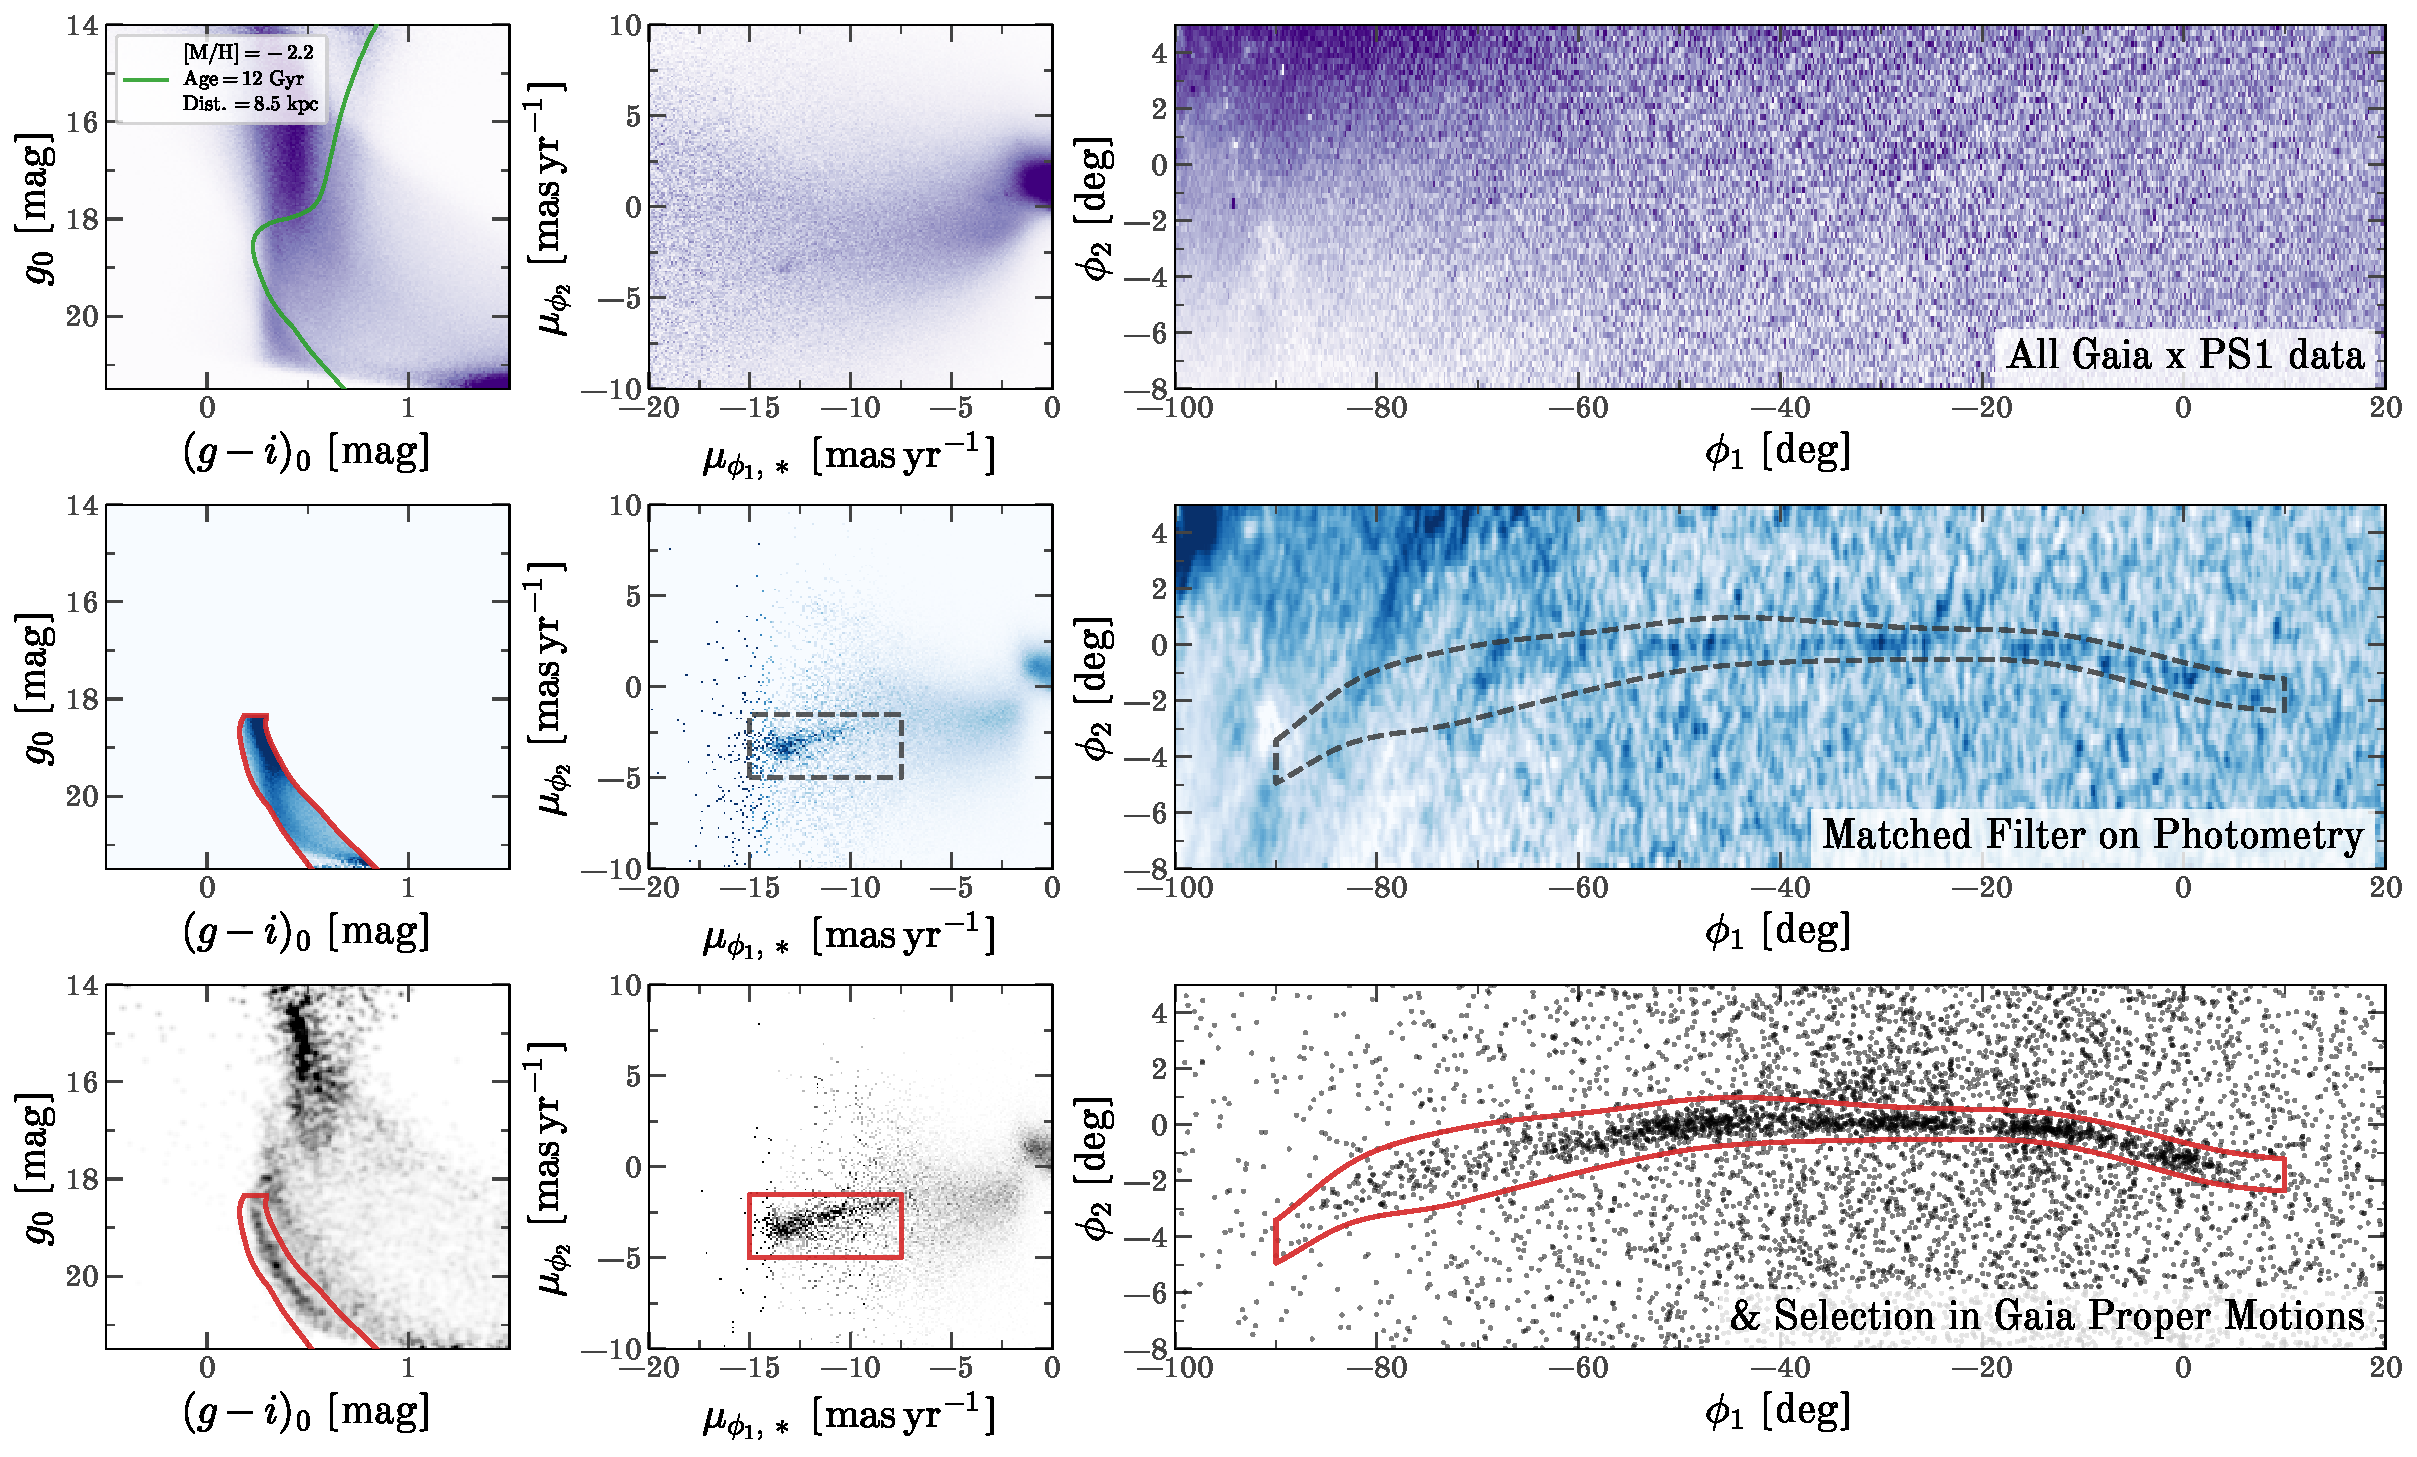
\includegraphics[width=1\textwidth]{gd1-filter-demo.pdf}
\end{center}
\caption{%
A demonstration ...
\textbf{Top row:}
\textbf{Middle row:}
\textbf{Bottom row:}
\label{fig:gd1-demo}
}
\end{figure*}

Figure~\ref{fig:gd1-demo} is a recreation of ... now using data from \gaia\ \dr{3} ...
which demonstrates the power of using \gaia\ astrometry to filter for stream members.
TODO: describe figure



- Until Gaia, total of XX streams reported.
- More dimensions = better contrast for finding low density things
- Greatly improved contrast for nearby streams (GD-1)
- Enabled more automated searches: streamfinder, Via Machinae, ... others??

- Challenge: Most streams are ~20 kpc, to MSTO out of Gaia magnitude limit

- Data from the \gaia\ Mission has revolutionized our ability to find kinematic substructures, led to the explosion in number of streams discovered
- Enabled by semi-automated methods - past methods stream-by-stream, natural evolution for a field
- New discoveries and census as of 2023
- Also: follow-up now more efficient so the chemistries now becoming more readily available

- list:
-- ED-2
-- LMS-1 / Wukong

- Clumps in dynamical quantities - student who worked with Robyn...


\subsection{Key opportunities}
- The point that (all - few) streams have MSTO below Gaia faint limit and what that does for density characterization (or in “stream structure” below?)
- (reorder by complexity, maybe :)): Automated discovery with quantified selection function, discovery in “hard” parts of parameter space (in the disk plane or galactic center, not tangent to sky plane, etc…), comparison to expectations from cosmological simulations and GC formation models


- Validation
- Truly automated detection - characterize selection effects
- Astrometry opportunities below Gaia limit (Rubin, Roman)
- Deeper photometry - main sequence but more contamination from phot alone
    - Combine with spectroscopy of full halo?

- In the future, hope to have fully automated methods to enable assessing selection function, population studies
- Still, Gaia not end-all, be-all -- faint limit is an issue (many streams found from photometric)


\section{Stream structure}
\label{sec:structure}
% APW
- Long known sagittarius bifurcation, no clear model to reproduce
- Now: Gaps and off-track features common at low surface brightness
- E.g., GD-1, Jhelum, AAU
- also motivated uncovering low-sb in other data sets (e.g., Pal 5, Jet, Phoenix)

- track--pm misalignments (shipp, erkal, ...)

\subsection{Key opportunities}
- density modeling robust to survey selection functions and dust


\section{Stream kinematics}
\label{sec:orbits}
% AB

- orbits!

- orbital statistics
- origin
- plane

- progenitors
- different parts of a whole

- targeting
- chemistries

% - a lot of what we want to do w streams is reconstructing their history
% - depends on orbit!
% - previously widely unknown (or rather, hard to get, so available for a few streams, but wildly unknown for most -- cite hermus hyllus stuff)
% -- hermus \citep{grillmair:2014}
% -- hermus, phoenix connection \citep{gc:2016}
% -- bhb sdss velocities -> different orbit of hermus, not connected w phoenix \citep{martin:2018}
%
% % - Still much unknown about most streams
% - But Gaia gives us access to kinematics -> +MW model = orbits
% - orbits good for:
% -- membership
% -- origin
% -- fitting the potential
% -- satellite encounters
%
% - better membership:
% -- S5 \citep{li:2022}
% -- new streamfinder paper
%
%
% - progenitors important: can model much better (kupper)
% - hard to find (balbinot)
% - before: only 2 gc streams
% - gjoll--ngc3201 chemistry \citep{hansen:2020}
%
% - gaia: low sb bc selecting on orbits
% - now a huge population, key opportunity
%
% - orbits also connected separately identified streams
% - case: oc
% - case: aau \citep{li:2021}
% - important for accurate accounting as we're moving to more complete census
%
% - more connections + benefit of orbits: phase-space clustering \citep{bonaca:2021}
% - found origins (accreted vs in situ) + progenitor galaxies
% - important for cocoon implications
%
% - orbital plane distribution, not aligned w the vpos \citep{riley:2020}

\subsection{Key opportunities}
- More comprehensive spectroscopic follow-up, potential modeling of a flexible potential, Stellar populations and element abundances, comparison to surviving dwarf galaxies and clusters (internal properties and orbits)
- high-precision kinematics of streams to distinguish perturbations
- figure: progenitor, bar, gmc, dm subhalo (sky, vr - sampled 100m/s, pm - sampled GDR5)


\section{Outlook}
\label{sec:outlook}
- Due to large number of streams: transitioning from stamp-collecting to population studies
- All of this will need improved theoretical modeling of the new Gaia discoveries (+ outlook for the future)
- Due to more secure membership probabilities: follow-up now more efficient so the chemistries now becoming more readily available


%% The Appendices part is started with the command \appendix;
%% appendix sections are then done as normal sections
%% \appendix

%% \section{}
%% \label{}


\bibliographystyle{model2-names-astronomy}
\bibliography{refs, apw-refs}

\end{document}

\endinput
%%
%% End of file `elsarticle-template-harv.tex'.
